\documentclass[a4paper,11pt]{article}
%\pdfoutput=1 % if your are submitting a pdflatex (i.e. if you have
             % images in pdf, png or jpg format)
\usepackage{jheppub} % for details on the use of the package, please
                     % see the JHEP-author-manual
\usepackage[T1]{fontenc} % if needed

\usepackage{slashed}
%\usepackage{subfigure}
\usepackage{xspace}
\usepackage{booktabs}
\author[a]{Federico Ambrogi}

% e-mail addresses: one for each author, in the same order as the authors\emailAdd{federico.ambrogi@oeaw.ac.at}
\emailAdd{federico.ambrogi88@gmail.com}

\newcommand{\dp}{\textit{dp}}
\newcommand{\rh}{\textit{rh}}
%% %simple case: 2 authors, same institution
%% \author{A. Uthor}
%% \author{and A. Nother Author}
%% \affiliation{Institution,\\Address, Country}


\title{\boldmath General Documentation}

\begin{document} 
	\sffamily
	\maketitle
	
	
	
\section{Common Data Model}
In this Section the information relative to the Common Data Model (CDM) are summarised.
\subsection{Convention Tables}
Table \ref{CDM} summarises the naming convention for the variables used in netCDF files (converted from the odb files with the \textit{readodbfile\_station.py} script).
The variable definition, their naming convention, and the physics units follow the preliminary CDM-common data model agreement, that can be found at:
\newline
\url{https://github.com/glamod/common_data_model/}
\newline
\url{https://github.com/glamod/common_data_model/blob/master/tables/observed_variable.dat}



%\input(a.tex) does not work on windows?


\begin{table}[!htbp]
	\footnotesize
	\begin{center}
		\renewcommand{\arraystretch}{1.3}
		\begin{tabular}{ l l l p{3.5in}}
			\toprule
			\textbf{Variable} & \textbf{CDM Name} & \textbf{Units} & \textbf{Description}  \\ \toprule \toprule
			pressure & pressure & [Pa] & pressure of air column at specified height\\
			dewpoint & dew point temperature & [K] & Dew point temperature is the temperature at which a parcel of air reaches saturation upon being cooled at constant pressure and specific humidity.\\
			wind & wind & [m s-1] & Speed is the magnitude of velocity. Wind is defined as a two-dimensional (horizontal) air velocity vector,  with no vertical component. (Vertical motion in the atmosphere has the standard name upward air velocity.) The wind speed is the magnitude of the wind velocity. Lot 1 uses ff  - WMO abbrev.\\
			humidity & specific humidity & [g kg-1] & specific means per unit mass. Specific humidity is the mass fraction of water vapor in (moist) air.\\
			\bottomrule \bottomrule
		\end{tabular}
	\end{center}
	\caption{Definition of naming convention, description and units for the variables contained in the netCDF files.}
	\label{CDM}
\end{table}

\clearpage
\section{Relative Humidity and Dew Point Temperature}
In this section the procedure to extract the relative humidity (\rh) and dew point temperature (\dp) is described.
The measured data for the rh and dp might be contained in the original odb file. In this case, as for the other variables such as air temperature and wind speed, the data is extracted directly from the odb files and converted to the netCDF format.
However the \rh or the \dp can be calculated from the other variable if the temperature is also known, using the saturation water vapor pressure.
\subsection{Equations}
 The formula known as \textit{FOEEWMO} (see the humidity.py script) gives the saturation water vapor pressure in Pascal:
\begin{equation}
FOEEWMO = 611.21 \times e^{17.502 \times \frac{t - 273.16}{t -32.19} } .
\end{equation}
The \rh temperature can be calculated as:
\begin{equation}
rh = \frac{FOEEWMO(dp)}{FOEEWMO(t)}
\end{equation}
i.e. evaluating the ratio of the saturation water vapor pressure at dew point temperature and at the measured air temperature. For the station 10939, which often reports directly both the \rh and \dp values, it was tested that the \rh measure values matched the values calculated using the formula above \footnote{Note that in the humidity.py script, the formula sh2rh allows to calculate the \rh from the specific humidity; however a discrepancy of constant factor $\sim$0.62 was found between the calculated and observed values.}.
\\
It is also possible to calculate the \dp knowing the \rh value by inverting the FOEEWMO formula as:
\begin{equation}
FOEEWMO(dp) = FOEEWMO(t) \times rh 
\end{equation}

\begin{equation*}
611.21 \times e^{17.502 \frac{dp - 273.16}{dp-32.19}} = FOEEWMO(t) \times rh
\end{equation*}

\begin{equation*}
 e^{17.502 \frac{dp - 273.16}{dp-32.19}} =  \frac{FOEEWMO(t) \times rh}{611.21}
\end{equation*}


\begin{equation*}
def \ F(t) \equiv \frac{FOEEWMO(t) \times rh}{611.21}
\end{equation*}


\begin{equation*}
 \frac{dp - 273.16}{dp-32.19} = \frac{ln \left( F(t) \right)}{17.502}   
\end{equation*}

\begin{equation*}
dp - 273.16 = \left(\frac{ln \left(  F(t) \right)}{17.502}   \right) \times dp - \frac{32.19}{17.502} \times ln \left(  F(t) \right)
\end{equation*} 

\begin{equation*}
dp - \left(\frac{ln \left(  F(t) \right)}{17.502}   \right) \times dp  = - \frac{32.19}{17.502} \times ln \left(  F(t) \right) + 273.16
\end{equation*} 


\begin{equation*}
\left (  1 - \frac{ ln \left(  F(t)  \right)}{17.502} \right) \times dp = - 1.839 \times ln \left(   F(t)    \right) + 273.16 
\end{equation*} 




\begin{equation}
dp =  \frac{ - 1.839 \times ln \left(   F(t)    \right) + 273.16 }{\left (  1 - \frac{ ln \left(  F(t)  \right)}{17.502} \right)}
\end{equation}


\subsection{Scripts}
All the scripts here described can be retrieved in \url{https://github.com/MBlaschek/CEUAS/tree/master/CEUAS/dev_federico/extract_Humidity_DewPoint}.
The aim is to analise the netCDF files, extracted from the odb files, regarding the relative humidity and dew point temperature. Whenever the data for these two variables is not available, the relative humidity will be calculated using the temperature and the dew point temperature. In principle it is possible to calculate relative humidity by using the specific humidity and the temperature, however this method results in unclear discrepancy, as it will be shown in Section \ref{comparison}.

\subsubsection{Description}
The script \verb|extract_Humidity_Temperature.py| reads the data contained in the files for temperature, humidity (specific and relative), and dew point temperature for a given observation station. The first element to check is that the datum available for each variable, i.e. the array of observation dates, is identical, since in principles they can be different. For example, some entries might be missing. In general the temperature data should always be present, and it is needed in order to extract the others. 
\\

The script then checks if the values of the relative humidity and dew points are available. If such values are available, there is nothing to be done. Otherwise, a new file called "\_calc\_sh\_rh\_dp.nc" is produced, containing a merged dataset with the original observation data, and calculated values for the missing entries. According to the \textbf{CDM} conventions, the variables are named "\textit{dew\_point\_temperatures}", "\textit{relative\_humidity}" and "\textit{specific\_humidity}". 
\\
To keep a record of the source of the data, an additional field with a prefix 'source\_' plus the name of the variable is added to the file. For each entry, the value '1' is assigned to observation data (or data from the odb file), and '2' to calculated values. 
\\
The functions used for the conversion of the variables are defined in the script called "humidity" . 



\subsubsection{FOEEWMO vs sh2rh} \label{comparison}
The \textbf{FOEEWMO} and \textbf{sh2rh} function allow for the calculation of the relative humidity, starting respectively from the dew point temperature and the specific humidity. The definition of such functions can be find in the document ECMWF IFS CY31R1 Data Assimilation Documentation (Page 86-88) at \url{https://www.ecmwf.int/en/elibrary/9225-part-ii-data-assimilation} .
The values of the relative humidity calculated with the two functions were tested against the observed data for the station 10393, since both the specific and relative humidity and the dew point temperature are available. Fig. \ref{ratio} shows that, while the FOEEWMO function reproduces accurately the values of the observed relative humidity, the function sh2rh gives a constant offsett of 0.62 . This is still under investigation.


\begin{figure}[!b]
	\centering
	\subfigure
	{ 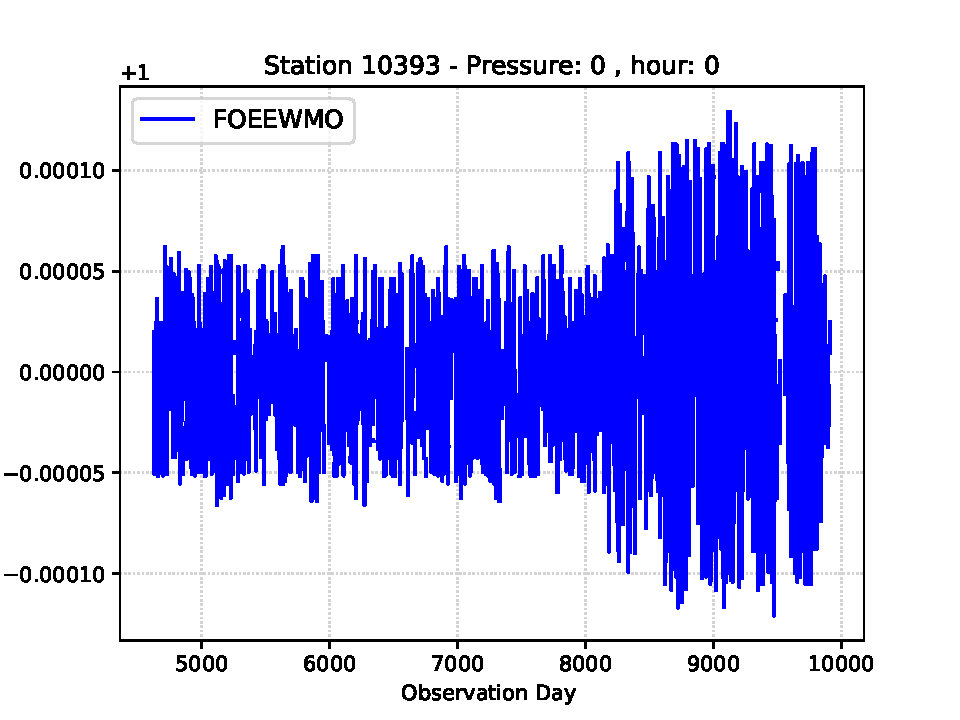
\includegraphics[width=0.49\textwidth]{Fig/ratios_FOEEWMO_0_0.pdf}}
	\subfigure
	{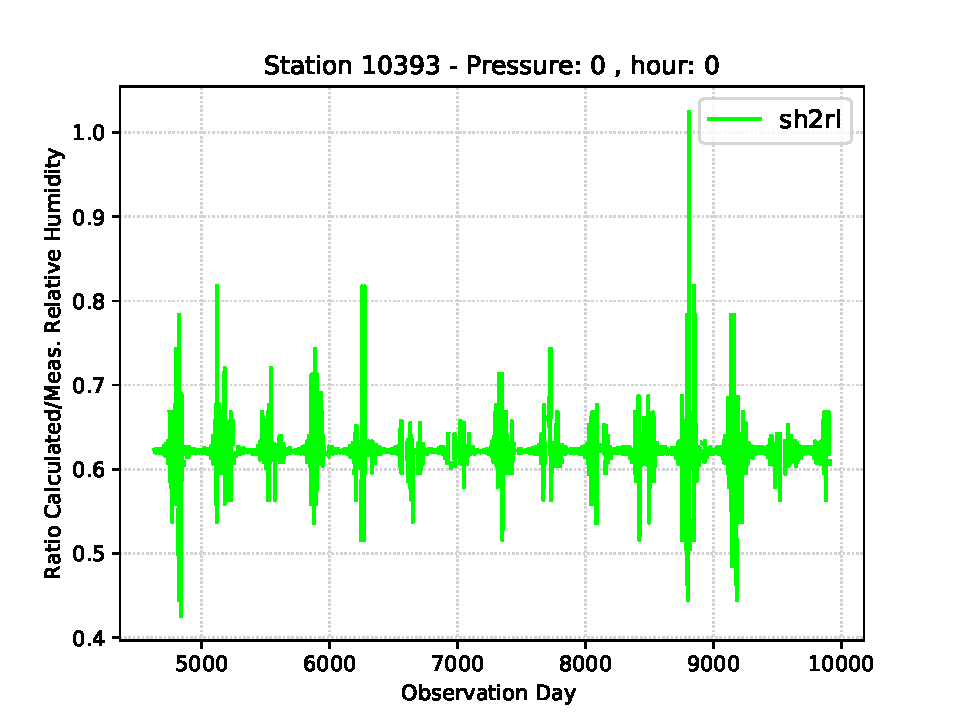
\includegraphics[width=0.49\textwidth]{Fig/ratios_sh2rl_0_0.pdf}}
	\caption{Ratio of the calculated versus observed relative humidity, using the FOEEWMO (left) and sp2rh (right) functions.}
	\label{ratio}
\end{figure}






% The following file contains the tables
% produced automatically by the CDM_Format.py file 



%\input(Tables.txt)

%\bibliographystyle{JHEP}
%\bibliography{references}


\end{document}



